\documentclass[../thesis-main.tex]{subfiles}

\begin{document}
\label{ch:litreview}
  \begin{quote}
   \emph{In this section, the relevant background information is given. This starts with a brief outline of the function and structure of the heart, ranging from the high order organisation of the heart into functional compartments, down to the cellular level. Further details are then given on the physiological aspects of some of the subcellular components of cardiac tissue. The evolution of computational models to describe the electrical activity of the heart is charted briefly, with special attention given to models specifically used in this thesis. Variation is then described, both in experimental and physiological measurements, and how this variation has been addressed in computational models. Then the pathological condition of isch\ae mia will be described, and the computational efforts to model this outlined.}
  \end{quote}


 \section{Cardiac Physiology}
 \label{sec:physiology}
 At the most general level, the heart serves as a pump to transport blood around the body to deliver nutrients and remove waste products. It does this by rhythmic, organised contraction---the rate of this contraction varies depending on species, age, condition of the heart and the activity being undertaken by the organism.
 
 \subsection{Structure of the Mammalian Heart}
 \label{subsec:heart-structure}
 \begin{figure}
  \centering
  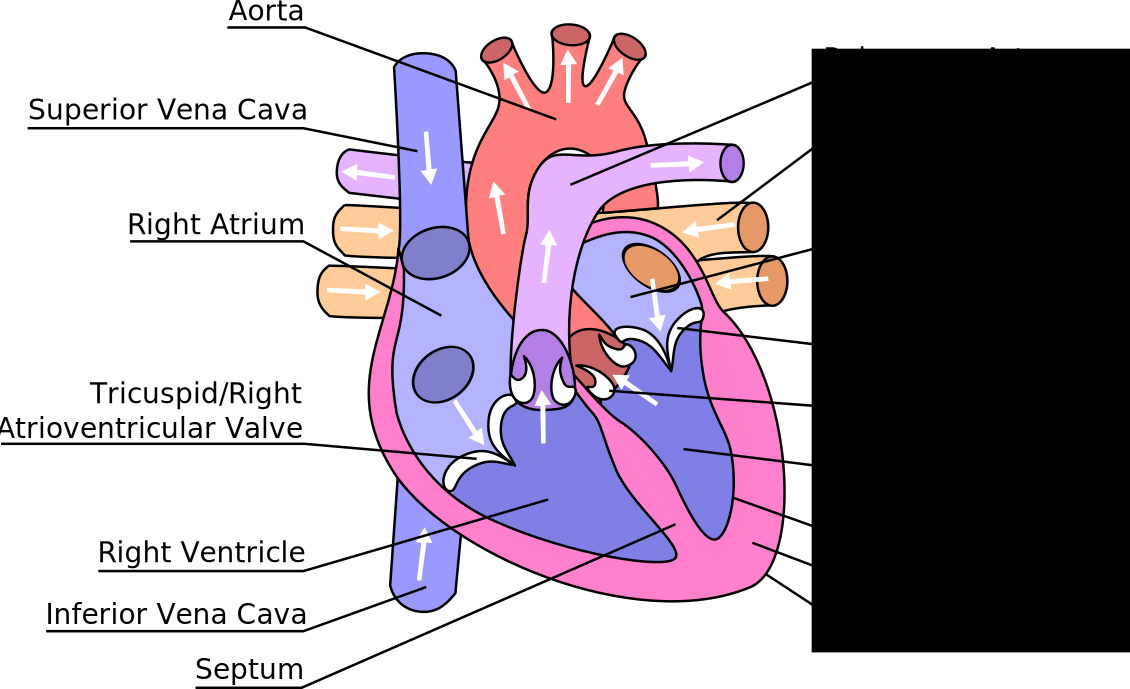
\includegraphics[width=0.75\textwidth]{heart_labels}
  \caption[Structure of the mammalian heart]{Diagram of the longitudinal cross-section of a mammalian heart. The direction of blood flow is shown by white arrows, and all major structural components are labelled.}
  \label{fig:heart-structure}
 \end{figure}
 Fig.~\ref{fig:heart-structure} shows the anatomical structure of the mammalian heart---while the size obviously varies widely between mammals, the overall architecture remains constant. It is split into two halves, left and right, by a muscular wall called the \emph{septum}, and then further subdivided into two chambers, the larger, lower chamber being a \emph{ventricle}, and the smaller, upper chamber called an \emph{atrium}.
 
 The passage of blood through the heart follows thus: firstly, deoxygenated blood from the body enters the heart via the superior and inferior/posterior \emph{vena cava}, with superior and inferior representing whether the blood comes from the upper or lower half of the body respectively. Via this channel, it enters the \emph{right atrium}. Passing through the \emph{tricuspid valve} (also known as the right atrioventricular valve), the blood enters the \emph{right ventricle}, where it is then pumped via the \emph{pulmonary artery} to the lungs, where it is oxygenated. The blood returns to the heart via the \emph{pulmonary vein}, entering the \emph{left atrium}, before moving through the \emph{mitral valve} (also known as the left atrioventricular valve) into the \emph{left ventricle}. The blood is then pumped via the \emph{aorta} to the rest of the body. The valves in the heart serve to ensure the flow of blood is always in the correct direction.
 
 The walls of the heart are mostly composed of muscular tissue known as \emph{myocardium}. The thickness of the myocardium is not constant throughout the heart, being thickest in the left ventricle, which requires the greatest force of contraction to pump the blood from the heart to the rest of the body. The myocardium can be split into three different regimes, as labelled in italics in Fig.~\ref{fig:heart-structure}: the \emph{epicardium} is the outermost layer of the myocardium, the \emph{midmyocardium} is the middle layer, and the \emph{endocardium} is the innermost layer. The cells composing these different layers possess different electrophysiological properties; the differences, and the consequences, will be expanded upon in \S\ref{subsec:electro-prop}.
 
 \begin{figure}
  \centering
  \begin{subfigure}[b]{0.45\textwidth}
   \centering
   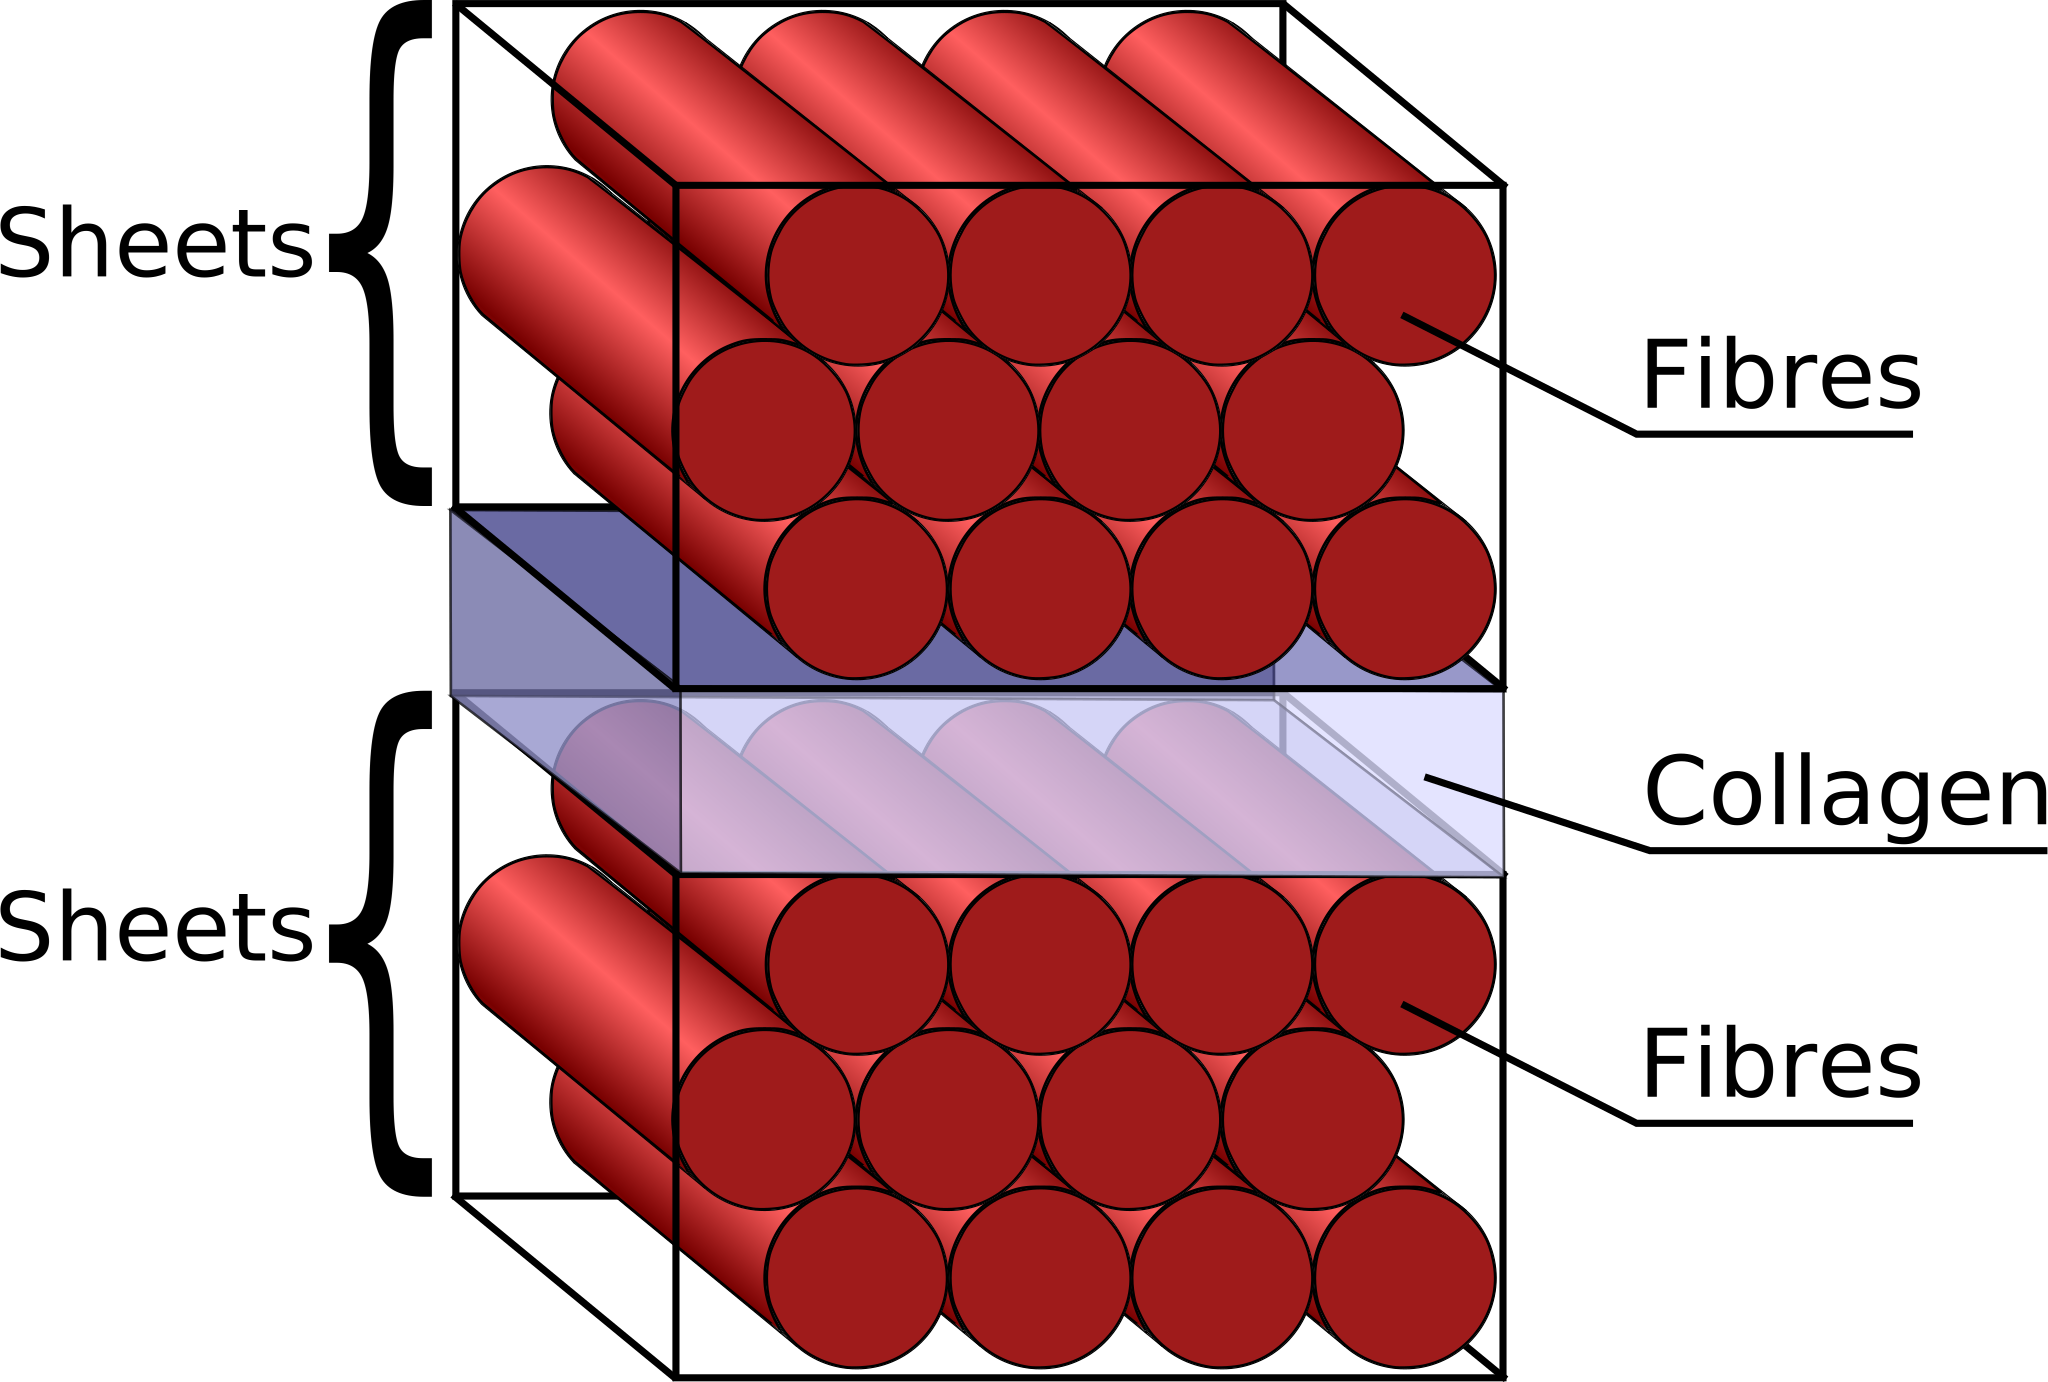
\includegraphics[width=\textwidth]{myocytes}
   \caption{Schematic}
   \label{subfig:myocyte-diagram}
  \end{subfigure}
  \begin{subfigure}[b]{0.45\textwidth}
   \centering
   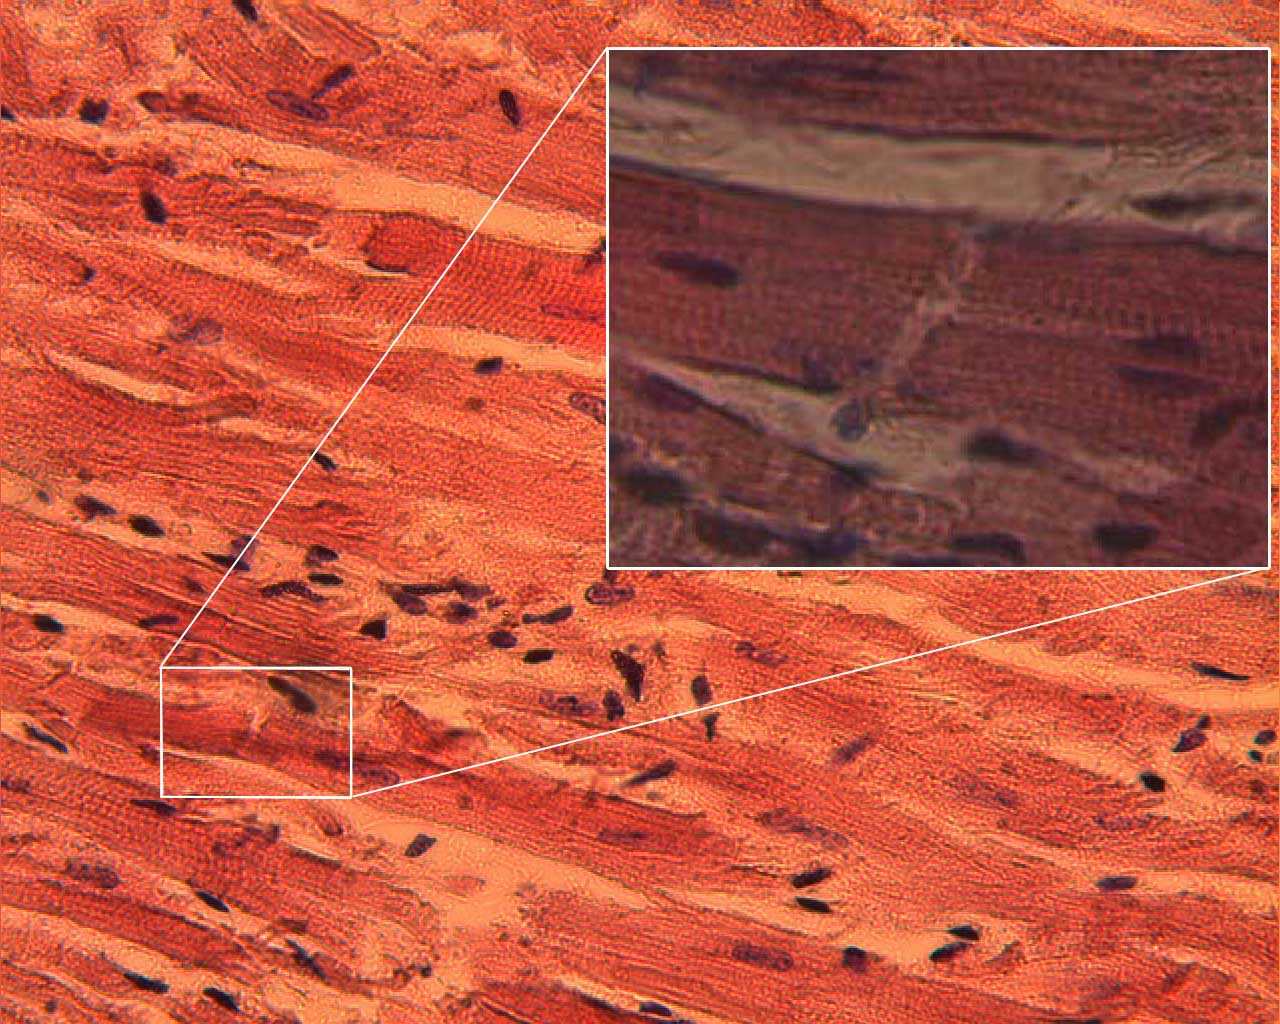
\includegraphics[width=\textwidth]{myocyte-image}
   \caption{Image}
   \label{subfig:myocyte-image}
  \end{subfigure}
  \caption[Structure of myocardial sheets and fibres]{(\ref{subfig:myocyte-diagram}) Schematic of the structure of myocardial sheets and fibres. (\ref{subfig:myocyte-image}) Image of cardiomyocytes demonstrating the interconnected nature of the individual myocytes into fibres.}
  \label{fig:myocyte-structure}
 \end{figure}
 
 The structure within the myocardium is shown in Fig.~\ref{subfig:myocyte-diagram}: it is composed of a series of sheets of tissue separated by collagen. The myocytes themselves lie longitudinally in these sheets to form fibres, with myocytes in the fibre direction connected to each other by intercalated discs (as opposed to skeletal muscle, which is composed of multinucleated fibres); this structure is seen in Fig.~\ref{subfig:myocyte-image}. One attribute of these discs is the presence of \emph{gap junctions}, which serve to electrically couple the myocytes by allowing ion flow between the two neighbouring myocytes in the fibre direction. This arrangement of the myocytes into electrically coupled fibres allows for coordinated contraction, and the fibrous structure allows the heart to twist as it contracts, leading to a more efficient pumping mechanism.
 
 The conduction pattern of the heart is key to the effective pumping mechanism---by controlling the sequence of electrical events in the heart, the sequence of conduction is similarly controlled. An outline of the conduction pattern of the heart is shown in Fig.~\ref{fig:conduction-pattern}. The sequence of activation starts amongst a group of self-excitatory cells at the top of the right atrium, called the \emph{sinoatrial node}. The action potential wave spreads from this node, causing the atrium to contract, before it reaches the \emph{atrioventricular node}---this is the only pathway for electrical excitation to pass from the atria to the ventricles. From the atrioventricular node, the excitation wave passes to the \emph{Bundle of His}, which conducts the electrical stimulus via the left and right bundle branches into the \emph{Purkinje system} near the bottom of the heart, which transmits the stimulus to the ventricular surface; as the stimulus has thus been transmitted directly from the atria to the bottom of the ventricles, the excitation wave thus spreads upwards through the ventricles, allowing the ventricles to contract from the bottom up as required.
 \begin{figure}
  \centering
  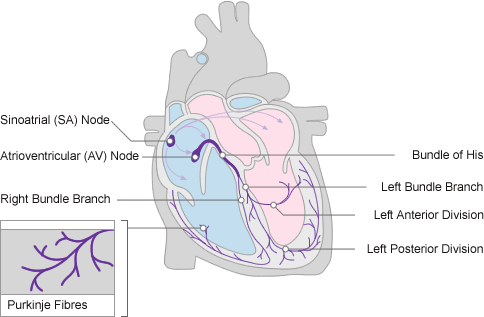
\includegraphics[width=0.8\textwidth]{cardiac_conduction}
  \caption[Pattern of electrical activation in the heart]{Schematic outline of the sequence of electrical activation in the mammalian heart. Image originally downloaded from www.nottingham.ac.uk on 10th December 2012.}
  \label{fig:conduction-pattern}
 \end{figure}
 
 \subsection{Electrophysiological Properties of Cardiomyocytes}
 \label{subsec:electro-prop}
 As previously stated, the main r\^ole of the heart is to serve as a pump to circulate the blood around the body. To do this effectively, it requires coordinated contraction, and this is achieved through the use of coupling the electrical activity of the heart of the mechanical activity (the details of this mechanism will be expanded upon in \S\ref{subsubsec:ecc}).
 
 Physically, cardiomyocytes are typically $10-20\mu$m in diameter, and $50-100\mu$m in length. They are cells bound by a lipid bilayer membrane, separating intracellular space (containing the cytoplasm, nuclei and other organelles) from the extracellular space. The intracellular space has a very different composition to the extracellular space, with the intracellular space containing a high and low concentration of potassium (\K) and sodium (\na) ions respectively; the reverse is true for the extracellular space. These concentration differences are the main reason behind their being a potential difference set up across the cell membrane, referred to as the \emph{membrane potential} ($V_m$). At rest, due to the high \K{} and low \na{} in the cell,this potential is negative, though the magnitude varies depending upon the location in the heart; a cardiomyocyte in the ventricles typically has a resting potential ($V$\sub{rest})) of about $-80$mV, while the sinoatrial node has a resting potential of between $-50$ and $-60$mV.
 
 Embedded within the bilayer are various membrane-bound proteins which serve to transport ions across the membrane, allowing the membrane to be selectively permeable to particular ions, and allowing regulation of this permeability as required. These transporters can be classed as either \emph{channels} (allow ions to move according to their electrochemical gradient), \emph{pumps} (translocate ions in the opposite direction to their electrochemical gradient by the use of energy) or \emph{exchangers} (translocates a number of ions of one type across the membrane in `exchange' for a number of ions of another type). Most of these transporters are ion-specific, though some are not exclusively selective. Most of these channels are also controlled by, amongst other things, the membrane potential itself \citep{Bezanilla2000}. The membrane potential causes a conformational change in the ion channel protein, causing it to `open' or `close', that is to allow ions to be conducted through it or not.
 
 These ion channels are discrete molecular entities, and thus the conformational changes that lead to their open/close state are stochastic; the effects of this stochasticity are discussed in greater detail in \S\ref{sec:param-var}. However, each type of ion channel possesses its own range of attributes, such as the time it takes to inactivate, the time it takes to reactivate, its permeability to different types of ions, and its susceptibility to other gating factors. Comprehensive summaries of the properties of ion channels is given in \citet{Carmeliet2002, Roden2002}.
 
 Electrically, the heart can be modelled with great success as an analogue to an electrical circuit \citep{Carmeliet2002}, where the lipid bilayer is represented as a capacitor, and the various ion channels and transporters that span the membrane are represented as resistors, which change their `resistance' depending on their state. By altering the resistance of these channels, ion flow across the membrane is permitted via an ionic current. It is a point of nomenclature that an `inward' current represents the movement of positive ions from the extracellular to the intracellular space, and an `outward' current is the reverse. This definition is based on the movement on electrical charge, and not on the movement of ion flow. This is subtly different to the definition of an inward or outward rectifier current, where an inward rectifier current passes current more easily inward than outward, and vice versa for an outward rectifier current.
 
 The changes in internal/external ion concentrations which result from these currents changes $V_m$. The cyclic, periodic change in membrane potential is referred to as the \emph{action potential} (AP). An example of an action potential, showing the different `phases', is shown in Fig.~\ref{fig:ap-structure}. 
 \begin{figure}
  \centering
  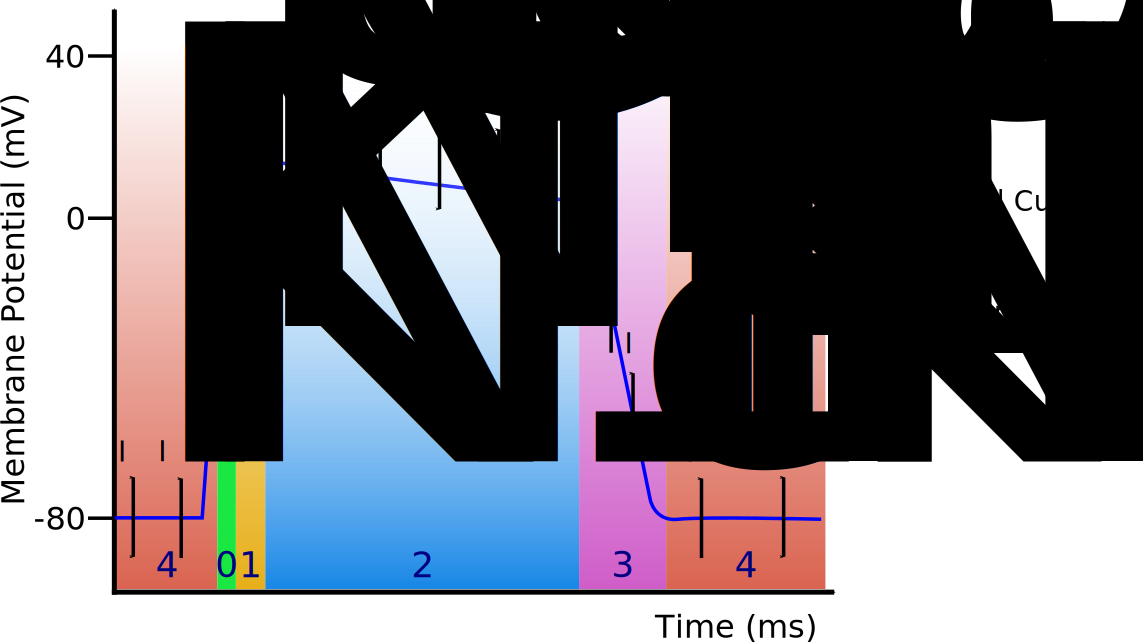
\includegraphics[width=0.8\textwidth]{ap-structure-full}
  \caption[Schematic of a cardiac AP]{Schematic of a ventricular cardiac AP, with the different `phases' of the AP shown, and which key currents are involved in each phase. Upward arrows represent outward currents, inward currents represent inward currents, and double arrows represent exchangers, \idest, where current moves in both an inward and outward direction.}
  \label{fig:ap-structure}
 \end{figure}
 
 The AP is considered to consist of 5 different phases, outlined below. The important currents in each phase are mentioned, and greater details are given for a number of these current in \S\ref{subsubsec:channel-dynamics}.
 \begin{description}
  \item[Phase 4:] The resting phase. For ventricular and atrial cardiomyocytes, this phase is marked by a relatively constant value for $V_m$. The negative resting potential is largely achieved by the inwardly rectifying potassium current (\ikix{}) remaining open during this phase. For pacemaker cells, \ikix{} is absent, and thus the resting phase is actually a period of slow depolarisation, until $V_m$ reaches the threshold value for phase 0. There is also an inward current due to the \na{}-\ca{} exchanger current (\inaca), which moves 3 \na{} ions into the cell and one \ca{} ion out at the resting potential.
  \item[Phase 0:] Period of rapid depolarisation that marks the start of the AP. It is initiated by $V_m$ reaching a threshold value which causes the \ina{} current to activate, causing a rapid influx of \na{} into the cell. The direction of \inaca{} reverses, and this newly outward current brings in \ca{} and removes \na{}.
  \item[Phase 1:] Transient repolarisation. The \na{} channels rapidly deactivate, and the activation of the transient \K{} outward current (\ito{}, occasionally referred to as $I_{\textnormal{to1}}$) results in a period of rapid, partial repolarisation. There may also be a contribution from a \ca{}-activated \cl (\icacl, or $I_{\textnormal{to2}}$). Depending on the strength of this current, this repolarisation may be to the extent that there is a `notch' in the AP. For example, there is a notch in the AP for ventricular epicardial cells, but no notch for ventricular endocardial cells. The characteristics of this phase are also species-dependent \citep{Carmeliet2006}.
  \item[Phase 2:] Plateau phase. The membrane potential is sustained at a relatively constant level by a balance of calcium (\ca{}) influx via the L-type calcium current (\ica{}), and potassium efflux, through the rectifier \K{} currents (rapid,\ikr{}, and slow, \iks{}). Despite being a rapidly activated current, \ikr{} does not carry large current early during this phase, but only peaks at the end. \ikix{} shows a dramatic fall in conductance during this phase. While most \ina{} is inactivated during phase 1, there is a small contribution from \ina{} when $V_m$ is in the limited range where activation and inactivation both occur. Late during phase 2, due to the increase in \cai{}, the reversal potential for \inaca{} increases to a value greater than $V_m$, and thus \inaca{} returns to being an inward current.
  \item[Phase 3:] Repolarisation. The L-type \ca{} current channels close, while the \iks{} channels remain open, allowing continuing \K{} efflux resulting in a repolarisation of the cell to the original resting potential. \ikix{} opens during this phase, to remain open during phase 4 to maintain a steady resting potential. 
 \end{description}
 It should be noted that the above description of which currents act during which phase is only an outline. While the upstroke of the AP is due mostly to the action of \ina{} and the associated rapid influx of \na{} ions into the cell, causing the rapid depolarisation, the remaining phases of the AP are more complex, and the failure or part failure of any individual component of the cell mechanism does not necessarily lead to the failure of the whole system. This pseudo-redundancy was first termed \emph{repolarisation reserve} in \citet{Roden1998}, and was demonstrated experimentally in \citet{Varro2000}. It is essentially the concept that a delay in repolarisation function caused by a reduction or loss of function in one repolarising current can be recovered by increased action of an alternative repolarising current. Most often, this term is applied to \K{} channels, and specifically for the interaction between \ikr{} and \iks{} \citep{Xiao2008}. Several currents are of noted for their r\^ole in maintaining the repolarisation reserve of the cell, some of which have already been mentioned: \ikr{}, \iks{}, \ikix{}, \ito{}, \ica{}, \ina{} \citep{Varro2011}. The repolarisation reserve is not constant, but rather is dynamic with pacing rate, and variable between species and tissues within the heart \citep{Carmeliet2006}.
 
 \subsubsection{Ion Channel Dynamics}
 \label{subsubsec:channel-dynamics} 
 \ikr{}, as the name implies, is the more rapidly activating of the two rectifier \K{} currents ($\tau\sim40$ms at $+30$mV), and rapidly activates once $V_m$ increases above $-30$mV. However, the channel inactivates even more rapidly in a process that precedes voltage-dependent inactivation \citep{Varro2011, Spector1996, Carmeliet2006}. Due to this, \ikr{} channels are largely closed during the plateau phase of the AP, only reopening when $V_m$ returns to about 0mV. The transient nature of the current is due to its rapid recovery from inactivation, and subsequent slow deactivation. At slow rates, the contribution of \ikr{} diminishes further, resulting in a positive feedback look regarding AP duration (APD) lengthening (the same is observed for \ikix{}) \citep{Virag2009}. This same vulnerability of the repolarisation is evident when depolarising factors (\eg, \ina{}, \ica{}) are augmented or repolarising factors (\eg, \iks{}, \ikix{}) diminished.
 
 If its function is impaired substantially in some way, APD is significantly prolonged by both direct measurements and QT interval measurements in electrocardiograms (ECGs)  (the QT interval serves as a marker for the time taken for ventricular depolarisation and repolarisation in a clinical setting), suggesting especial importance in cellular repolarisation \citep{Varro2000, Lengyel2001, Jost2005}. When \ikr{} is only impaired in a minor way, APD may not necessarily increase due to the action of the repolarisation reserve. \ikr{} is due to a channel encoded by the human ether-\'a-go-go related gene (HERG), and is known for being its susceptibility to the effects of drug block, making it of key pharmocological importance \citep{Vandenberg2001, Haverkamp2000}.
 
 \iks{} takes longer to activate than its partner (500-1000ms at plateau phase), and deactivates rapidly at negative $V_m$ \citep{Jost2005, Varro2011}. Its carries a slowly rising current over the duration of the plateau phase. At rapid pacing rates, the current carried by the \iks{} channel increases---this is thought to be due to the kinetics of the channel, with an `inactivated' state being intermediate between the open and closed state. At rapid pacing rates, there is less time to transition fully to the closed state, and thus there is a greater proportion of \iks{} channels available for immediate opening \citep{Silva2005}.
 
 Drug block of \iks{} does cause AP prolongation, but not to the same extent as \ikr{}; while direct measurements show a slight increase in APD, there is very little or no change in QT intervals ECG measurements \citep{Varro2000, Lengyel2001, Jost2005}. This implies that its amplitude, compared to that of \ikr{}, during a typical AP is small---this has been confirmed experimentally under normal conditions \citep{Varro2011}. Combined with its slow activation, there is thus relatively little \iks{} active during the AP \citep{Jost2005}. However, its long activation time also means the effect of \iks{} block is more pronounced APD is prolonged, due to (i) the net outward current at long pacing rates is smaller, so the fractional effect of \iks{} is greater, and (ii) more channels are activated during a long AP \citep{Carmeliet2006}. Due to this action, and the response of \iks{} to sympathetic stimulation, the current provides a negative feedback for APD prolongation, acting to curtail the increased action of \ica{} that occurs at longer pacing rates. Thus, while under `normal' circumstances \iks{} has limited effect on the repolarisation reserve of the cell, it acts as an effective buffer when APD is longer than normal.
 
 The transmural differences in the expression of \iks{} is a large reason behind the transmural variation of APD, and also explains why \ikr{} block can have a greater or lesser effect, depending on the abundance of the compensatory effect of \iks \citep{Vandenberg2001, Carmeliet2006}. The density of \iks{} channels has also been shown to increase in response to sustained \ikr{} block, demonstrating its importance to the repolarisation reserve \citep{Xiao2008}.
 
 \ikix{} is a strongly inwardly rectifying \K{} current, which means that when $V_m$s is greater than $-30$mV, the channel is inactivated. Thus it plays a negligible r\^ole during the plateau phase of the AP, but has a self-reinforcing role in the repolarisation of the cell once $V_m$ decreases to the extent that \ikix{} can be activated. It should be noted that this is not a voltage-dependent activation, but is based on an unblocking of the channel: when $V_m > -30$mV, the channel is blocked by \mg{} and polyamines which enter the channel from the intracellular side in a voltage-dependent manner. As the current is fully open at $V$\sub{rest}, it resists depolarisation caused by either increased pacemaker activity, or \ca{} overload-related delayed afterdepolarisations (DADs). Consequently, \ikix{} may be considered to play an unusual r\^ole in the repolarisation reserve, and impairment of its function could lead to proarrhythmic effects by making the cell more susceptible to extrasystoles.
 
 \ito{} is actually composed of two separate currents, a rapidly recovering component (\itof{}) and a slowly recovering component (\itos{}). As a combined unit, it both activates and inactivates rapidly for $V_m > -20$mV, and is of greatest importance during the phase 1 repolarisation. As such, it is believed to have little influence directly on the end repolarisation of the cell, but due to its early role, and its consequent effect on the plateau potential, it is believed to have influence on subsequent currents, which lead to great indirect influence. \ito{} is also known for its transmural variation, being greater in epicardial than endocardial tissue.
 
 \inak{} is caused due to the \na{}-\K{} pump, which is an electrogenic exchanger, moving 3 \na{} ions out of the cell in exchange for 2 \K{} ions. It thus works to maintain the concentration gradients and the resting membrane potential, and provides an outward current in support of the repolarisation reserve. It is, however, sensitive to intracellular \na{} concentration (\nai), and consequently to the rate of stimulation.
 
 The influence of \ica{} on the repolarisation of the cell is complex due to its complicated inactivation. It inactivates due to voltage slowly, and thus the main reason for its inactivation is due to \ca{}-induced inactivation, and is thus in response to local \ca{} concentration, which is dynamically changing during the plateau phase. This inactivation is modulated via a protein called calmodulin, and thus can be modulated further. If the AP is extended during the range of activation/inactivation for \ica{}, some \ica{} channels may reactivate. This resurgence of the inward current can lead to secondary depolarisations or early after-depolarisations (EADs) \citep{Carmeliet2006}. 
 
 If \ica{} (or \ina{}) are augmented and have their activity increased, this serves to make the plateau potential more positive. While at first glance this may indicate that AP may lengthen, it is rather the case that this may serve to enhance activation of outward \K{} currents, thus shortening APD.
 
 The \na{}-\ca{} exchange current (\inaca{}, also referred to as \incx{}), like \inaca, is an electrogenic exchanger, this time exchanging 3 \na{} ions for one \ca{} ion. By this process, it is, with the SERCA pump, largely responsible for restoring the low cytosolic \ca{} concentration during diastole. It depends strongly on $V_m$ and \cai{}, and thus its magnitude during the AP is difficult to estimate (a problem compounded by the lack a specific inhibitor for the current). It is an outward current at the start of the AP, when $V_m$ and \cai{} are both low, but then changes to an inward current during the late plateau phase. Due to its sensitivity to \cai{}, in times of \ca{}-overload \inaca{} can provide a depolarising current, thus increasing the likelihood of DADs and EADs. The density of \ina{} is also known to depend heavily on \cai{}, decreasing when \cai{} is high; the gating of the channel is not affected.
 
 \subsubsection{Excitation-Contraction Coupling}
 \label{subsubsec:ecc}
 Arguably, the complex electrical activity of the AP just described exists for the sole purpose of ensuring the heart acts as an effective mechanical pump. As such, the linking of the electrical activity of the heart to its mechanical contraction is vital, as is referred to as \emph{excitation-contraction coupling}. What follows is a brief summary of the mechanism of this link (the reverse side of this mechanism, termed mechanoelectric feedback, shall not be discussed here).
 
 For this discussion, the cell may be decomposed into units called calcium release units (CRUs), also known as dyads \citep{Cleemann1998}. These CRUs are spread roughly evenly throughout the cell to allow for a uniform action throughout---the number of CRUs in the cell has been estimated to be between 10,000 and 100,000 \citep{Cleemann1998,Greenstein2002}. Anatomically, the CRU may be considered to be a section of the cell containing a section of the cell membrane, with some L-type \ca{} channels, and a section of the sarcoplasmic reticulum (SR). The primary r\^ole of the SR is to sequester and release \ca{} via ryanodine receptors (RyRs) when the required stimulus is given. This stimulus is the rise in local concentration of \ca{} precipitated by the opening of the L-type \ca{} current channels, and is termed \emph{calcium-induced calcium release}. The result is that a great deal of \ca{} is released into the cytosol of the cell during phase 2 of the AP. The reason this is vital for ECC is due to the interaction between \ca{} and the contractile units of the cell, called the sarcomere. When the cytosolic concentration of \ca{} (\cai{}) rises, the free \ca{} binds to a part of the contractile machinisms of the cell, which then removes the inhibition between the two critical contractile parts of the mechanism, allowing contraction to take place. Subsequently, the \ca{} released from the SR is recovered by the sarco/endoplasmic reticulum \ca{}-ATPase pumps \citep{Franzini-Armstrong2005}.
 
 \section{Computational Cell Models}
 \label{sec:cell-models}
 It is often not practicable to test hypotheses in full experimental conditions. In such times, computational/mathematical models have become of increasing importance in recent years, as they have developed from their original humble origins. Depending on the requirements of the model, great advances have been made in accurately modelling individual ion channels, assessing the importance of stochasticity, to probing the interplay between systems and levels in complicated simulations. What follows is a brief background on the evolution and development of computational cell models from their early days in \S\ref{subsec:model-development}, and then a summary of some of the key concepts that are of use in these models in \S\ref{subsec:model-concepts}.
 
 \subsection{Development}
 \label{subsec:model-development}
 What follows is a summary of the progression and development of computational cardiac models. For further details of the models themselves, the reader is referred to the original papers, and for more in depth summaries of the development, the reader is referred to the reviews given in \citet{Noble2001, Noble2012, Noble2011, Puglisi2004, Rudy2006, Niederer2009}.
 
 The precursor to all computational models of cardiac cells was the model developed in \citet{Hodgkin1952}. This model described the electrical acitivity of a giant squid axon. It described the ionic currents required to explain the change in membrane potential, using a model for each current of a series of activation and inactivation gating variables (details given in \S\ref{subsec:model-concepts}). This model was able to sufficiently model the AP of the neuron using only three ionic currents: a \K{} current, a \na{} current, and a `leak' current of other ions. It was further developed by \citet{Fitzhugh1960}, which even then recognised that, while the `truth' of the model was not universally accepted, the model nonetheless was successful in reproducing experimental results. However, FitzHugh was able to demonstrate that, with the correct adaptations of the model equations, the output could be altered to reproduce the longer APs of cardiac cells.
 
 The Hodgkin-Huxley model was hugely successful, and paved the way for the extension of the computational modelling approach to cardiac cells. Preliminary work was shown in \citet{Noble1960}, which presented an adaptation of the Hodgkin-Huxley model for the AP of cardiac pacemaker cells. The same 3 currents were used, with adaptations in \ik{} to reproduce the longer AP of cardiac cells. The model was subsequently refined and expanded to reproduce the AP of Purkinje fibre cells \citep{Noble1962}, taking into account experimental data demonstrating the existence of at least two \K{} currents (labelled $I$\sub{K}~and $I$\sub{K1}) with the resulting change in \K{} permeabilities of the cell membrane \citep{Hutter1960, Carmeliet1961, Hall1963}.
 
 This model was followed by a model designed to reproduce the AP of a ventricular myocyte \citep{Krause1966}. The Noble and Krause models were both based on the Hodgkin-Huxley model, with the Noble model being used as the seed for future developments in the computational cardiac modelling field. The next major refinement of the model came with that proposed by \citet{McAllister1975}. In response to experimental data, this model greatly expanded the number of ion channels that were being modelled---the previous 4 ODEs of the Noble model were now replaced with 10. This included modelling the componenets of \ik{} separately as \ikr{} and \iks{}, as well as incorporating a \ca{} current based on experimental recordings from patch clamp experiments. This model, despite its success in reproducing experimental data, also contained an impressive flaw, in that it posited the slow conductance changes near the resting potential to an outward current, activated by depolarisation. In fact, the change was due to an inward current activated by hyperpolarisation (the so-called `pacemaker current' (\iF)). Despite this flaw, the overall model remained sound, and iterations of the current continued through to \citet{DiFrancesco1985}, which was the first model to incorporate a formulation for the \na{}-\K{} exchanger, and made most intracellular ion concentrations dynamics. It also managed to model SR \ca{} release, and demonstrated the stoichiometry of the \na{}-\ca{} exchanger had to be 3:1, not 2:1 as had previously been supposed---consequently, the resulting current from this exchange (\inaca{}) was incorporated into future models.
 
 While this progress was still being made in the modelling of Purkinje fibre APs, a new focus was found in modelling the AP of ventricular myocytes. While this had already been achieved to some extent in \citet{Krause1966}, the first widely used ventricular model was that proposed in the work of \citet{Beeler1977}. This model was also the first to make more explicit mention of the internal calcium dynamics of the cell, by simulating the \ca{} release from the sarcoplasmic reticulum. Of particular note in the further development of the field is the so-called Luo-Rudy model, first published in \citet{Luo1991}. This model was originally designed to study arrhythmias in guinea pig ventricular cells, but has been subsequently developed for a wide variety of different tasks, and key components have been adapted into other models for other species \citep{Shaw1997a, Shaw1997b, Wagner1999, Viswanathan1999, Garfinkel2000, Shannon2004, Mahajan2008}. Specifically, the model was further adapted in two papers \citep{Luo1994, Luo1994a} to include dynamic intracellular ion concentrations, and \ica{} was reformulated. Significantly, \ik{} was separated into the two constituent currents of \ikr{} and \iks{} in \citet{Zeng1995}, based on experimental evidence for this separation \citep{Sanguinetti1990}. The Luo-Rudy model was also adapted to be able to model isch\ae mia by the incorporation of \ikatp{} \citep{Shaw1997} (further details of the modelling of isch\ae mia can be found in \S\ref{sec:ischaemia}). A further significant advance came with \citet{Clancy1999}, which for the first time incorporated Markov modelling into a cell model (Markov modelling is described in greater detail in \S\ref{subsubsec:markov}).
 
 It should be noted that almost all currents in the models described above still use the some basic model form as that given in \citet{Hodgkin1952}---details and nuances have been added to some equations, and other equations have been formulated using entirely different methods (\eg, Markov modelling), but the underlying modelling philosophy has remained rather steady, and been found sufficient to the present day.
 
 It is through this evolution of models from relatively humble beginnings that we have reached the point where we are today---computational models of cardiac systems can be used to model anything from the subcellular to the full organ level, with specialisations depending on species, location and situation. In this thesis, focus is mainly devoted to the models presented in \citet{Shannon2004} and \citet{Mahajan2008}. These are both models for rabbit ventricular myocytes, with the latter model being itself based on the former---they are both in turn based in large part on the Luo-Rudy model. However, it should not be thought that it is a direct lineage from the Luo-Rudy model to the Shannon model to the Mahajan model---there are numerous intervening steps \citep{Zeng1995, Puglisi2001, Bassani2004}.
 
 \subsection{Key Concepts}
 \label{subsec:model-concepts}
 The model's purpose defines what variables are considered, and how these variables are determined. Some models (\eg, citet{Restrepo2008}) define a certain section of the cellular mechanism as of interest, and thus the output is defined accordingly. However, most models are trained according to the membrane potential, and thus that is considered the primary output. In modelling the cell as an electrical circuit with the membrane considered as a capacitor, the instantaneous change in membrane potential is calculated according to
 \begin{equation}
  \frac{\textnormal{d}V_m}{\textnormal{d}t} = -\frac{1}{C_m}(I_{ion}+I_{stim}),
 \end{equation}
 where $C_m$ is the membrane capacitance, $I_{ion}$ is the sum of all ionic currents in and out of the cell, and $I_{stim}$ is the stimulus current, if applied, to initiate an AP.
 
 In biophysically detailed models of electrically excitable cells, most ionic currents are modelled according to:
 \begin{equation}
  I_X = g_X(\mathbf{x})(V_m-E_X),
 \end{equation}
 where $I_X$ represents the ionic current being modelled, $g_X(\mathbf{x})$ represents the conductance of the channel and $E_X$ represents the reversal potential of the cell, which is the potential at which there is no net ion flow through the channel, \idest, there will be no ionic current. The general form of $E_X$ is explained in \S\ref{subsubsec:nernst}. $g_X(\mathbf{x})$ is current-dependent variable, and can be modelled as varying with time, voltage, extra-/intracellular ion concentration, etc..
 
 \subsubsection{Nernst Potential}
 \label{subsubsec:nernst}
 Of key importance in mathematical modelling of electrically active cells is the \emph{Nernst equation}. A full derivation is given in the appendix, but the key result is thus:
 \begin{equation}
  E_X = \frac{RT}{z_XF}\ln\frac{[X]_\textnormal{o}}{[X]_\textnormal{i}}
 \end{equation}
 In the above equation, $R$ represents the gas constant, $z_X$ represents the valence of ion $X$, $F$ represents the Faraday constant, and $[X]_\textnormal{o}$ and $[X]_\textnormal{o}$ represent the extracellular and intracellular concentrations of $X$ respectively. The quantity of interest, $E_X$ is the \emph{Nernst potential} or \emph{reversal potential}, and represents the value of $V_m$ required to maintain the intra-/extracellular concentration ratio constant, \idest, to make the net ionic flux across the cell membrane zero.
 
 When a channel is entirely selective, the reversal potential (which can now be thought of as the potential at which there will be no net flux of ions) is given by the Nernst equation for the specific ion. However, some ion channels are permeable to more than one type of ion, in which case their reversal potential for channel $\alpha$ is given by the \emph{Goldman-Hodgkin-Katz equation}:
 \begin{equation}
  E_\alpha = \frac{RT}{F}\ln\frac{\Sigma_i^N P_{A_i^+}[A_i^+]_\textnormal{o} + \Sigma_j^M P_{B_j^-}[B_j^-]_\textnormal{i}}{\Sigma_i^N P_{A_i^+}[A_i^+]_\textnormal{i} + \Sigma_j^M P_{B_j^-}[B_j^-]_\textnormal{o}}
 \end{equation}
 The above equation describes the situation for $N$ different monovalent positive ionic species and $M$ monovalent negative ionic species; different valencies complicate matters further.In it, $E_\alpha$ represents the reversal potential for the channel, \idest, the potential at which, with the given ion concentrations, no net electric flow will occur. The permeability of the membrane is given by $P_X$; as with the concentrations, the terms have been split into positive ($A_i^+$) and negative ($B_i^-$) ionic terms.
 
 \subsubsection{Hodgkin-Huxley Current}
 As previously stated, the seminal work presented in \citet{Hodgkin1952} modelled currents as being composed of one of more activation/inactivation gates. It should be noted that the original paper was at pains to emphasise that this was not intended as a description of the actual, physical channel, but was to be used as is: as a mathematical equation that provides a fidelity to the experimental data.
 
 Within this framework, the current conductance can be modelled according to
 \begin{equation}
  g_X = \overline{g}_Xm^a h^b,
 \end{equation}
 where $\overline{g}_X$ represents the maximum conductance through the channel, $a$ and $b$ are constants, $m$ represents the activation gate and $h$ the inactivation gate. In \citet{Hodgkin1952}, a physical basis was given to $m$ and $h$ by describing them as proportions of `activating molecules' and `inactivating molecules', respectively---the conductance through the channel is thus proportional to the proportion of these molecules that are within and outwith the cell. The variation can thus be described according to
 \begin{equation}
  \frac{\textnormal{d}m}{\textnormal{d}t} = \alpha_m(1-m)-\beta_m,
 \end{equation}
 where $\alpha_m$ and $\beta_m$ are functions of $V_m$. It can be noted that this is often expressed as
 \begin{equation}
  \frac{\textnormal{d}m}{\textnormal{d}t} = \frac{m_\infty-m}{\tau_m}
 \end{equation}
 where $m_\infty=\frac{\alpha_m}{\alpha_m+\beta_m}$ and $\tau_m=\frac{1}{\alpha_m+\beta_m}$, and are the steady state value of $m$ and the time constant, respectively.
 
 At a basic level, in mathematical models of ion channel currents, it is assumed that, instantaneously, they behave like Ohmic resistors, \idest
 
 \subsubsection{Markov Models}
 \label{subsubsec:markov}
 The Hodgkin-Huxley formulation is computationally efficient, but does not represent a physical reality of the channel state. As such, it is poorly suited to model state specific processes, such as mutation effects or stochasticity. To overcome this, \emph{Markov modelling} can be used (it should be noted that in the formalism presented here, it is not suited to modelling stochastic processes, but can be adapted to do so). Markov modelling works by assuming that the channel can exist in any one of $n$ discrete states. These states can be open, closed or inactivated, and there can be multiple types of each state. The simplest form is a two state system, such as
 \begin{center}
  \ce{C <=>[\ce{$k_\textnormal{on}$}][\ce{$k_\textnormal{off}$}] O},
 \end{center}
 where $k_\textnormal{on}$ and $k_\textnormal{off}$ represent the transition rates between these two states---in cardiac modelling, these transition rates typically depend only on the membrane potential. The key requirement for a Markov model is the \emph{Markov property}, which states that the transition to the next state depends only on the current state, and there is no cumulative history of the system that influences its future. Thus, if $x_i(t)$ represents the proportion of channels in state $i$ at time $t$, and $k_{ij}$ represents the transition rate from state $i$ to state $j$, the transition rates for a system containing $m$ different states may be modelled according to
 \begin{equation}
  \frac{\textnormal{d}x_i}{\textnormal{d}t} = \sum_{j=1}^m (k_{ji}x_j - k_{ij}x_i).
 \end{equation}
 The conductance of the channels for a particular current is thus calculated by multiplying the maximum conductance by the proportion of the channels that currently exist in an open state.
 
 \section{Variation}
 \label{sec:param-var}
 Stochasticity has been mentioned in passing already in this dissertation. Stochasticity, and more generally variation, is now being recognised as being of key importance in many biological questions. Variation exists at all ranges, and at all scales---if one wished to be pedantic, one could point to the probabilistic collapse of the quantim wavefunction as the seed for all uncertainty, but there is no current evidence that quantum effects play any r\^ole in cardiac function. However, variation does exist, and accounting for it is becoming an increasingly important aspect of cardiac modelling.
 
 In \S\ref{subsec:experimental-var}, the various possible sources and problems of variation in biological settings are discussed, and in \S\ref{subsec:comp-var}, the various methods used so far to address this variation in computational models are outlined.
 
 \subsection{Experimental \& Physiological Variation}
 \label{subsec:experimental-var}
 As stated, variation exists at all scales, both temporally and spatially: from individual ion channels, to the level of the cell, to tissue, to organ, and to organism. At the scale of ion channels, this variation can be felt two-fold: 
 
 \subsection{Computational Modelling of Variation}
 \label{subsec:comp-var}
 Computationally, how much account of the variation at which scale must be made depends on the question being made, and the model being constructed to answer this question; in constructing a whole organ model of the heart to simulate the spread of the AP when considering fibre effects, there is likely little to no benefit in incorporating stochasticity at the level of ion channels.
 
 \section{Isch\ae mia}
 \label{sec:ischaemia}
 Despite what would be expected from the Nernst equation, increased extracellular \K{} is known to enhance \ikr{} \citep{Sanguinetti1992, Yang1997}
 
\end{document}
